% Copyright (c) 2010 Jérémie DECOCK (http://www.jdhp.org)

\documentclass[pdftex,a4paper,11pt]{article} 
\usepackage[utf8]{inputenc}
\usepackage[frenchb]{babel}
\usepackage[pdftex]{graphicx}
\usepackage{hyperref}

\hypersetup{
    pdftoolbar=true,                                          % show Acrobat’s toolbar ?
    pdfmenubar=true,                                          % show Acrobat’s menu ?
    pdffitwindow=true,                                        % page fit to window when opened
    pdftitle={Spécifications générales},                      % title
    pdfauthor={Jérémie DECOCK},                               % author
    pdfsubject={Spécifications générales},                    % subject of the document
    pdfnewwindow=true,                                        % links in new window
    pdfkeywords={},                                           % list of keywords
    colorlinks=true,                                          % false: boxed links; true: colored links
    linkcolor=black,                                          % color of internal links
    citecolor=black,                                          % color of links to bibliography
    filecolor=black,                                          % color of file links
    urlcolor=black                                            % color of external links
}

\begin{document}

\title{OpenCAL - Java\\\medskip
       Spécifications générales}
\author{Jérémie \bsc{Decock}}
\date{\today}

\maketitle

%%%%%%%%%%%%%%%%%%%%%%%%%%%%%%%%%%%%%%%%%%%%%%%%%%

\section{Diagrammes UML}
\subsection{Cas d'utilisation de l'application}

\begin{figure}[htbp]
    \centering
    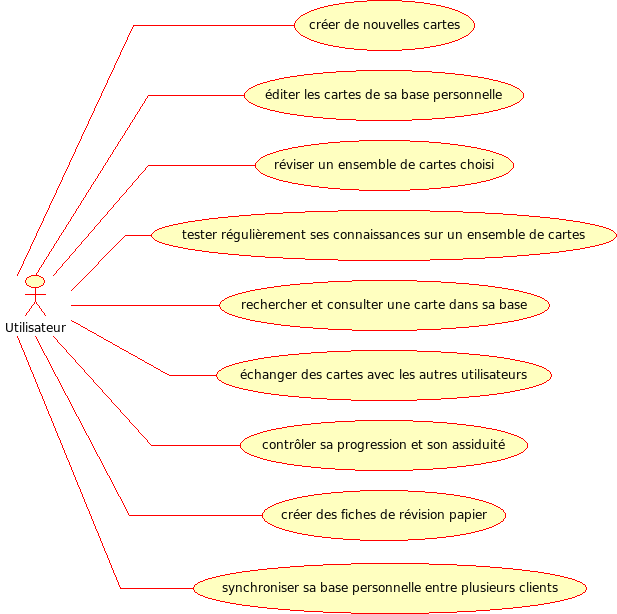
\includegraphics[width=10cm]{diagrams/use_case_diagram}
    \caption{Cas d'utilisation de l'application}
    \label{use_case}
\end{figure}

%%%%%%%%%%%%%%%%%%%%%%%%%%%%%%%%%%%%%%%%%%%%%%%%%%

\clearpage

\begin{center}
    Copyright \textcopyright{} 2010 Jérémie \bsc{Decock}.\\
    All right reserved.
\end{center}

\end{document}
